% Generated by Sphinx.
\def\sphinxdocclass{report}
\documentclass[letterpaper,10pt,openany,oneside]{sphinxmanual}
\usepackage[utf8]{inputenc}
\DeclareUnicodeCharacter{00A0}{\nobreakspace}
\usepackage[T1]{fontenc}
\usepackage[english]{babel}
\usepackage{times}
\usepackage[Bjarne]{fncychap}
\usepackage{longtable}
\usepackage{sphinx}
\usepackage{multirow}


\title{Concept: The Data Decomposition Pattern}
\date{July 18, 2014}
\release{}
\author{CSInParallel Project}
\newcommand{\sphinxlogo}{}
\renewcommand{\releasename}{}
\makeindex

\makeatletter
\def\PYG@reset{\let\PYG@it=\relax \let\PYG@bf=\relax%
    \let\PYG@ul=\relax \let\PYG@tc=\relax%
    \let\PYG@bc=\relax \let\PYG@ff=\relax}
\def\PYG@tok#1{\csname PYG@tok@#1\endcsname}
\def\PYG@toks#1+{\ifx\relax#1\empty\else%
    \PYG@tok{#1}\expandafter\PYG@toks\fi}
\def\PYG@do#1{\PYG@bc{\PYG@tc{\PYG@ul{%
    \PYG@it{\PYG@bf{\PYG@ff{#1}}}}}}}
\def\PYG#1#2{\PYG@reset\PYG@toks#1+\relax+\PYG@do{#2}}

\expandafter\def\csname PYG@tok@gd\endcsname{\def\PYG@tc##1{\textcolor[rgb]{0.63,0.00,0.00}{##1}}}
\expandafter\def\csname PYG@tok@gu\endcsname{\let\PYG@bf=\textbf\def\PYG@tc##1{\textcolor[rgb]{0.50,0.00,0.50}{##1}}}
\expandafter\def\csname PYG@tok@gt\endcsname{\def\PYG@tc##1{\textcolor[rgb]{0.00,0.25,0.82}{##1}}}
\expandafter\def\csname PYG@tok@gs\endcsname{\let\PYG@bf=\textbf}
\expandafter\def\csname PYG@tok@gr\endcsname{\def\PYG@tc##1{\textcolor[rgb]{1.00,0.00,0.00}{##1}}}
\expandafter\def\csname PYG@tok@cm\endcsname{\let\PYG@it=\textit\def\PYG@tc##1{\textcolor[rgb]{0.25,0.50,0.56}{##1}}}
\expandafter\def\csname PYG@tok@vg\endcsname{\def\PYG@tc##1{\textcolor[rgb]{0.73,0.38,0.84}{##1}}}
\expandafter\def\csname PYG@tok@m\endcsname{\def\PYG@tc##1{\textcolor[rgb]{0.13,0.50,0.31}{##1}}}
\expandafter\def\csname PYG@tok@mh\endcsname{\def\PYG@tc##1{\textcolor[rgb]{0.13,0.50,0.31}{##1}}}
\expandafter\def\csname PYG@tok@cs\endcsname{\def\PYG@tc##1{\textcolor[rgb]{0.25,0.50,0.56}{##1}}\def\PYG@bc##1{\setlength{\fboxsep}{0pt}\colorbox[rgb]{1.00,0.94,0.94}{\strut ##1}}}
\expandafter\def\csname PYG@tok@ge\endcsname{\let\PYG@it=\textit}
\expandafter\def\csname PYG@tok@vc\endcsname{\def\PYG@tc##1{\textcolor[rgb]{0.73,0.38,0.84}{##1}}}
\expandafter\def\csname PYG@tok@il\endcsname{\def\PYG@tc##1{\textcolor[rgb]{0.13,0.50,0.31}{##1}}}
\expandafter\def\csname PYG@tok@go\endcsname{\def\PYG@tc##1{\textcolor[rgb]{0.19,0.19,0.19}{##1}}}
\expandafter\def\csname PYG@tok@cp\endcsname{\def\PYG@tc##1{\textcolor[rgb]{0.00,0.44,0.13}{##1}}}
\expandafter\def\csname PYG@tok@gi\endcsname{\def\PYG@tc##1{\textcolor[rgb]{0.00,0.63,0.00}{##1}}}
\expandafter\def\csname PYG@tok@gh\endcsname{\let\PYG@bf=\textbf\def\PYG@tc##1{\textcolor[rgb]{0.00,0.00,0.50}{##1}}}
\expandafter\def\csname PYG@tok@ni\endcsname{\let\PYG@bf=\textbf\def\PYG@tc##1{\textcolor[rgb]{0.84,0.33,0.22}{##1}}}
\expandafter\def\csname PYG@tok@nl\endcsname{\let\PYG@bf=\textbf\def\PYG@tc##1{\textcolor[rgb]{0.00,0.13,0.44}{##1}}}
\expandafter\def\csname PYG@tok@nn\endcsname{\let\PYG@bf=\textbf\def\PYG@tc##1{\textcolor[rgb]{0.05,0.52,0.71}{##1}}}
\expandafter\def\csname PYG@tok@no\endcsname{\def\PYG@tc##1{\textcolor[rgb]{0.38,0.68,0.84}{##1}}}
\expandafter\def\csname PYG@tok@na\endcsname{\def\PYG@tc##1{\textcolor[rgb]{0.25,0.44,0.63}{##1}}}
\expandafter\def\csname PYG@tok@nb\endcsname{\def\PYG@tc##1{\textcolor[rgb]{0.00,0.44,0.13}{##1}}}
\expandafter\def\csname PYG@tok@nc\endcsname{\let\PYG@bf=\textbf\def\PYG@tc##1{\textcolor[rgb]{0.05,0.52,0.71}{##1}}}
\expandafter\def\csname PYG@tok@nd\endcsname{\let\PYG@bf=\textbf\def\PYG@tc##1{\textcolor[rgb]{0.33,0.33,0.33}{##1}}}
\expandafter\def\csname PYG@tok@ne\endcsname{\def\PYG@tc##1{\textcolor[rgb]{0.00,0.44,0.13}{##1}}}
\expandafter\def\csname PYG@tok@nf\endcsname{\def\PYG@tc##1{\textcolor[rgb]{0.02,0.16,0.49}{##1}}}
\expandafter\def\csname PYG@tok@si\endcsname{\let\PYG@it=\textit\def\PYG@tc##1{\textcolor[rgb]{0.44,0.63,0.82}{##1}}}
\expandafter\def\csname PYG@tok@s2\endcsname{\def\PYG@tc##1{\textcolor[rgb]{0.25,0.44,0.63}{##1}}}
\expandafter\def\csname PYG@tok@vi\endcsname{\def\PYG@tc##1{\textcolor[rgb]{0.73,0.38,0.84}{##1}}}
\expandafter\def\csname PYG@tok@nt\endcsname{\let\PYG@bf=\textbf\def\PYG@tc##1{\textcolor[rgb]{0.02,0.16,0.45}{##1}}}
\expandafter\def\csname PYG@tok@nv\endcsname{\def\PYG@tc##1{\textcolor[rgb]{0.73,0.38,0.84}{##1}}}
\expandafter\def\csname PYG@tok@s1\endcsname{\def\PYG@tc##1{\textcolor[rgb]{0.25,0.44,0.63}{##1}}}
\expandafter\def\csname PYG@tok@gp\endcsname{\let\PYG@bf=\textbf\def\PYG@tc##1{\textcolor[rgb]{0.78,0.36,0.04}{##1}}}
\expandafter\def\csname PYG@tok@sh\endcsname{\def\PYG@tc##1{\textcolor[rgb]{0.25,0.44,0.63}{##1}}}
\expandafter\def\csname PYG@tok@ow\endcsname{\let\PYG@bf=\textbf\def\PYG@tc##1{\textcolor[rgb]{0.00,0.44,0.13}{##1}}}
\expandafter\def\csname PYG@tok@sx\endcsname{\def\PYG@tc##1{\textcolor[rgb]{0.78,0.36,0.04}{##1}}}
\expandafter\def\csname PYG@tok@bp\endcsname{\def\PYG@tc##1{\textcolor[rgb]{0.00,0.44,0.13}{##1}}}
\expandafter\def\csname PYG@tok@c1\endcsname{\let\PYG@it=\textit\def\PYG@tc##1{\textcolor[rgb]{0.25,0.50,0.56}{##1}}}
\expandafter\def\csname PYG@tok@kc\endcsname{\let\PYG@bf=\textbf\def\PYG@tc##1{\textcolor[rgb]{0.00,0.44,0.13}{##1}}}
\expandafter\def\csname PYG@tok@c\endcsname{\let\PYG@it=\textit\def\PYG@tc##1{\textcolor[rgb]{0.25,0.50,0.56}{##1}}}
\expandafter\def\csname PYG@tok@mf\endcsname{\def\PYG@tc##1{\textcolor[rgb]{0.13,0.50,0.31}{##1}}}
\expandafter\def\csname PYG@tok@err\endcsname{\def\PYG@bc##1{\setlength{\fboxsep}{0pt}\fcolorbox[rgb]{1.00,0.00,0.00}{1,1,1}{\strut ##1}}}
\expandafter\def\csname PYG@tok@kd\endcsname{\let\PYG@bf=\textbf\def\PYG@tc##1{\textcolor[rgb]{0.00,0.44,0.13}{##1}}}
\expandafter\def\csname PYG@tok@ss\endcsname{\def\PYG@tc##1{\textcolor[rgb]{0.32,0.47,0.09}{##1}}}
\expandafter\def\csname PYG@tok@sr\endcsname{\def\PYG@tc##1{\textcolor[rgb]{0.14,0.33,0.53}{##1}}}
\expandafter\def\csname PYG@tok@mo\endcsname{\def\PYG@tc##1{\textcolor[rgb]{0.13,0.50,0.31}{##1}}}
\expandafter\def\csname PYG@tok@mi\endcsname{\def\PYG@tc##1{\textcolor[rgb]{0.13,0.50,0.31}{##1}}}
\expandafter\def\csname PYG@tok@kn\endcsname{\let\PYG@bf=\textbf\def\PYG@tc##1{\textcolor[rgb]{0.00,0.44,0.13}{##1}}}
\expandafter\def\csname PYG@tok@o\endcsname{\def\PYG@tc##1{\textcolor[rgb]{0.40,0.40,0.40}{##1}}}
\expandafter\def\csname PYG@tok@kr\endcsname{\let\PYG@bf=\textbf\def\PYG@tc##1{\textcolor[rgb]{0.00,0.44,0.13}{##1}}}
\expandafter\def\csname PYG@tok@s\endcsname{\def\PYG@tc##1{\textcolor[rgb]{0.25,0.44,0.63}{##1}}}
\expandafter\def\csname PYG@tok@kp\endcsname{\def\PYG@tc##1{\textcolor[rgb]{0.00,0.44,0.13}{##1}}}
\expandafter\def\csname PYG@tok@w\endcsname{\def\PYG@tc##1{\textcolor[rgb]{0.73,0.73,0.73}{##1}}}
\expandafter\def\csname PYG@tok@kt\endcsname{\def\PYG@tc##1{\textcolor[rgb]{0.56,0.13,0.00}{##1}}}
\expandafter\def\csname PYG@tok@sc\endcsname{\def\PYG@tc##1{\textcolor[rgb]{0.25,0.44,0.63}{##1}}}
\expandafter\def\csname PYG@tok@sb\endcsname{\def\PYG@tc##1{\textcolor[rgb]{0.25,0.44,0.63}{##1}}}
\expandafter\def\csname PYG@tok@k\endcsname{\let\PYG@bf=\textbf\def\PYG@tc##1{\textcolor[rgb]{0.00,0.44,0.13}{##1}}}
\expandafter\def\csname PYG@tok@se\endcsname{\let\PYG@bf=\textbf\def\PYG@tc##1{\textcolor[rgb]{0.25,0.44,0.63}{##1}}}
\expandafter\def\csname PYG@tok@sd\endcsname{\let\PYG@it=\textit\def\PYG@tc##1{\textcolor[rgb]{0.25,0.44,0.63}{##1}}}

\def\PYGZbs{\char`\\}
\def\PYGZus{\char`\_}
\def\PYGZob{\char`\{}
\def\PYGZcb{\char`\}}
\def\PYGZca{\char`\^}
\def\PYGZam{\char`\&}
\def\PYGZlt{\char`\<}
\def\PYGZgt{\char`\>}
\def\PYGZsh{\char`\#}
\def\PYGZpc{\char`\%}
\def\PYGZdl{\char`\$}
\def\PYGZti{\char`\~}
% for compatibility with earlier versions
\def\PYGZat{@}
\def\PYGZlb{[}
\def\PYGZrb{]}
\makeatother

\begin{document}

\maketitle
\tableofcontents
\phantomsection\label{index::doc}


\textbf{Prologue}

This document contains reading material that introduces a classic and ubiquitous
pattern used in parallel programs: \textbf{data decomposition}.
Programs containing this pattern perform computations over elements of data
stored in linear data structures (and potentially other types of data structures; but we will stick to linear here).  In non-parallel, or `serial', or `sequential' implementations of programs that contain linear data structures, we often iterate over all the data elements using a for loop. In parallel implementations, we need to decide which elements will be computed by multiple processing units at the same time. We dub the choices we make in our parallel implementation for achieving this the \textbf{data decomposition pattern}, because we will chose a decomposition, or mapping of elements in the data structure to processing units available to us.  We introduce an
example analogous to ``Hello World'' for this data decomposition programming pattern:
addition of vectors, using the simple linear array data structure.  We have code examples for different types of hardware and software that enable parallel computation.

The first two chapters introduce the problem and describe ways to decompose it onto processing units.  The next three chapters show examples of just how this is done for three different hardware and software combinations. We wrap up with alternative mapping schemes and some questions for reflection.

\textbf{Nomenclature}

A \textbf{Processing Unit} is an element of software that can execute instructions on hardware.  On a multicore computer, this would be a \emph{thread} running on a core of the multicore chip.  On a cluster of computers, this would be a \emph{process} running on one of the computers. On a co-processor such as a Graphics Processing Unit (GPU), this would be a \emph{thread} running on one of its many cores.

A program that uses only one procesing unit is referred to as a \emph{serial} or \emph{sequential} solution. You are likely most familiar with these types of programs.

\textbf{Prerequisites}
\begin{itemize}
\item {} 
Knowledge of C programming language is helpful.

\item {} \begin{description}
\item[{Basic understanding of three types of parallel and distributed computing (PDC) hardware:}] \leavevmode\begin{itemize}
\item {} 
Shared-memory multicore machines

\item {} 
Clusters of multiple computers connected via high-speed networking

\item {} 
Co-processor devices, such as graphical processing units (GPU)

\end{itemize}

\end{description}

\item {} \begin{description}
\item[{Though not strictly necessary, if you want to compile and run the code examples, you will need unix-based computers with:}] \leavevmode\begin{itemize}
\item {} 
MPI installed on a single computer or cluster (either MPICH2 or OpenMPI)

\item {} 
gcc with OpenMP (most versions of gcc have this enabled already) and a multicore computer

\item {} 
CUDA developer libraries installed on a machine with a CUDA-capable GPU

\end{itemize}

\end{description}

\end{itemize}

We have compiled and run these on linux machines or clusters with a few different GPU cards.

\textbf{Code Examples}

You can download \code{VectorAdd.tgz} to obtain all of the code examples shown in the following sections of this reading.


\chapter{Vector Addition}
\label{VectorAdd/VectorAddProblem:concept-the-data-decomposition-pattern}\label{VectorAdd/VectorAddProblem::doc}\label{VectorAdd/VectorAddProblem:vector-addition}
The problem we will examine is this: we wish to add each element of vector A with its corresponding element in vector B and placing the sum of the two elements in its corresponding location in vector C.  This example problem has sometimes been called the ``Hello, World'' of parallel programming. The reasons for this are:
\begin{itemize}
\item {} 
the sequential implementation of the code is easy to understand

\item {} 
the pattern we employ to split the work is used many times in many situations in parallel programming

\end{itemize}

Once you understand the concept of splitting the work that we illustrate in this example, you should be able to use this pattern in other situations you encounter.

The problem is quite simple and can be illustrated as follows:
\begin{figure}[htbp]
\centering

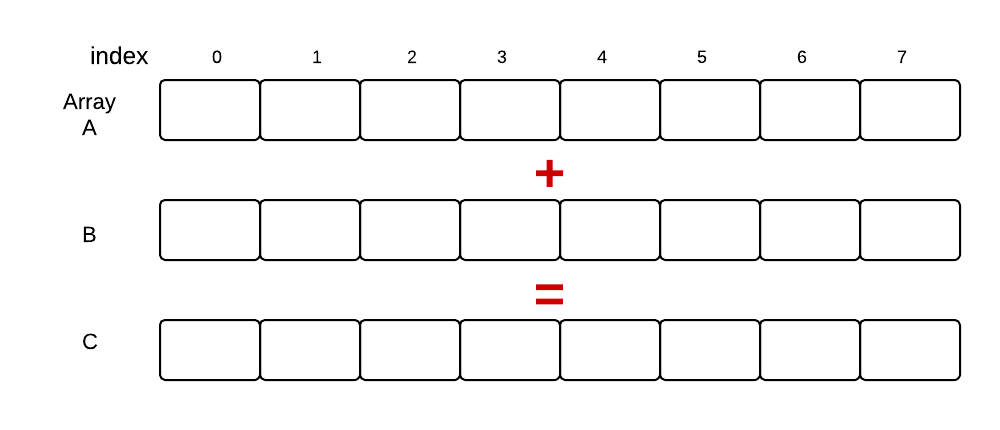
\includegraphics{VectorAdditionProblem.png}
\end{figure}

We have two arrays, A and B, and array C will contain the addition of corresponding elements in A and B. In this simple example we are illustrating very small arrays containing 8 elements each.  Suppose those elements are integers and A and B had the following elements in it:
\begin{figure}[htbp]
\centering

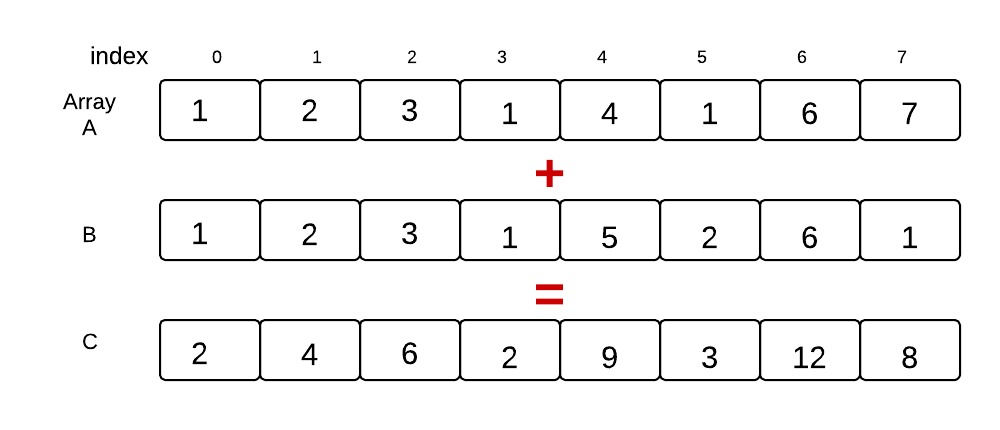
\includegraphics{VecAddSolution.png}
\end{figure}

The elements in array C above depict the result of adding a vector as stored in array A to a vector as stored in array  B.

We use very small vectors of size 8 for illustration purposes. A sequential solution to this problem, written in C code, is found in the file named \textbf{VectorAdd/Serial/VA-sequetial.c} in the compressed tar file of examples that accompanies this reading. It looks like this:

\begin{Verbatim}[commandchars=\\\{\},numbers=left,firstnumber=1,stepnumber=1]
\PYG{c+cp}{\PYGZsh{}}\PYG{c+cp}{include \PYGZlt{}stdlib.h\PYGZgt{}   }\PYG{c+c1}{//malloc and free}
\PYG{c+cp}{\PYGZsh{}}\PYG{c+cp}{include \PYGZlt{}stdio.h\PYGZgt{}    }\PYG{c+c1}{//printf}

\PYG{c+cp}{\PYGZsh{}}\PYG{c+cp}{define ARRAY\PYGZus{}SIZE 8     }\PYG{c+c1}{//Size of arrays whose elements will be added together.}

\PYG{c+cm}{/*}
\PYG{c+cm}{ *  Classic vector addition.}
\PYG{c+cm}{ */}
\PYG{k+kt}{int} \PYG{n+nf}{main} \PYG{p}{(}\PYG{k+kt}{int} \PYG{n}{argc}\PYG{p}{,} \PYG{k+kt}{char} \PYG{o}{*}\PYG{n}{argv}\PYG{p}{[}\PYG{p}{]}\PYG{p}{)} 
\PYG{p}{\PYGZob{}}
	\PYG{c+c1}{// elements of arrays a and b will be added}
	\PYG{c+c1}{// and placed in array c}
	\PYG{k+kt}{int} \PYG{o}{*} \PYG{n}{a}\PYG{p}{;}
	\PYG{k+kt}{int} \PYG{o}{*} \PYG{n}{b}\PYG{p}{;} 
	\PYG{k+kt}{int} \PYG{o}{*} \PYG{n}{c}\PYG{p}{;}
        
        \PYG{k+kt}{int} \PYG{n}{n} \PYG{o}{=} \PYG{n}{ARRAY\PYGZus{}SIZE}\PYG{p}{;}   \PYG{c+c1}{// number of array elements}
	\PYG{k+kt}{int} \PYG{n}{i}\PYG{p}{;}       \PYG{c+c1}{// loop index}
        
        \PYG{c+c1}{// allocate spce for the arrays}
        \PYG{n}{a} \PYG{o}{=} \PYG{p}{(}\PYG{k+kt}{int} \PYG{o}{*}\PYG{p}{)} \PYG{n}{malloc}\PYG{p}{(}\PYG{k}{sizeof}\PYG{p}{(}\PYG{k+kt}{int}\PYG{p}{)}\PYG{o}{*}\PYG{n}{n}\PYG{p}{)}\PYG{p}{;}
	\PYG{n}{b} \PYG{o}{=} \PYG{p}{(}\PYG{k+kt}{int} \PYG{o}{*}\PYG{p}{)} \PYG{n}{malloc}\PYG{p}{(}\PYG{k}{sizeof}\PYG{p}{(}\PYG{k+kt}{int}\PYG{p}{)}\PYG{o}{*}\PYG{n}{n}\PYG{p}{)}\PYG{p}{;}
	\PYG{n}{c} \PYG{o}{=} \PYG{p}{(}\PYG{k+kt}{int} \PYG{o}{*}\PYG{p}{)} \PYG{n}{malloc}\PYG{p}{(}\PYG{k}{sizeof}\PYG{p}{(}\PYG{k+kt}{int}\PYG{p}{)}\PYG{o}{*}\PYG{n}{n}\PYG{p}{)}\PYG{p}{;}

        \PYG{c+c1}{// initialize arrays a and b with consecutive integer values}
	\PYG{c+c1}{// as a simple example}
        \PYG{k}{for}\PYG{p}{(}\PYG{n}{i}\PYG{o}{=}\PYG{l+m+mi}{0}\PYG{p}{;} \PYG{n}{i}\PYG{o}{\PYGZlt{}}\PYG{n}{n}\PYG{p}{;} \PYG{n}{i}\PYG{o}{+}\PYG{o}{+}\PYG{p}{)} \PYG{p}{\PYGZob{}}
            \PYG{n}{a}\PYG{p}{[}\PYG{n}{i}\PYG{p}{]} \PYG{o}{=} \PYG{n}{i}\PYG{p}{;}
        \PYG{p}{\PYGZcb{}}
        \PYG{k}{for}\PYG{p}{(}\PYG{n}{i}\PYG{o}{=}\PYG{l+m+mi}{0}\PYG{p}{;} \PYG{n}{i}\PYG{o}{\PYGZlt{}}\PYG{n}{n}\PYG{p}{;} \PYG{n}{i}\PYG{o}{+}\PYG{o}{+}\PYG{p}{)} \PYG{p}{\PYGZob{}}
            \PYG{n}{b}\PYG{p}{[}\PYG{n}{i}\PYG{p}{]} \PYG{o}{=} \PYG{n}{i}\PYG{p}{;}
        \PYG{p}{\PYGZcb{}}   
        
        \PYG{c+c1}{// Compute the vector addition}
        \PYG{k}{for}\PYG{p}{(}\PYG{n}{i}\PYG{o}{=}\PYG{l+m+mi}{0}\PYG{p}{;} \PYG{n}{i}\PYG{o}{\PYGZlt{}}\PYG{n}{n}\PYG{p}{;} \PYG{n}{i}\PYG{o}{+}\PYG{o}{+}\PYG{p}{)} \PYG{p}{\PYGZob{}}
		\PYG{n}{c}\PYG{p}{[}\PYG{n}{i}\PYG{p}{]} \PYG{o}{=} \PYG{n}{a}\PYG{p}{[}\PYG{n}{i}\PYG{p}{]}\PYG{o}{+}\PYG{n}{b}\PYG{p}{[}\PYG{n}{i}\PYG{p}{]}\PYG{p}{;}
        \PYG{p}{\PYGZcb{}}
	
	\PYG{c+c1}{// Check for correctness (only plausible for small vector size)}
	\PYG{c+c1}{// A test we would eventually leave out}
	\PYG{n}{printf}\PYG{p}{(}\PYG{l+s}{"}\PYG{l+s}{i}\PYG{l+s+se}{\PYGZbs{}t}\PYG{l+s}{a[i]}\PYG{l+s+se}{\PYGZbs{}t}\PYG{l+s}{+}\PYG{l+s+se}{\PYGZbs{}t}\PYG{l+s}{b[i]}\PYG{l+s+se}{\PYGZbs{}t}\PYG{l+s}{=}\PYG{l+s+se}{\PYGZbs{}t}\PYG{l+s}{c[i]}\PYG{l+s+se}{\PYGZbs{}n}\PYG{l+s}{"}\PYG{p}{)}\PYG{p}{;}
        \PYG{k}{for}\PYG{p}{(}\PYG{n}{i}\PYG{o}{=}\PYG{l+m+mi}{0}\PYG{p}{;} \PYG{n}{i}\PYG{o}{\PYGZlt{}}\PYG{n}{n}\PYG{p}{;} \PYG{n}{i}\PYG{o}{+}\PYG{o}{+}\PYG{p}{)} \PYG{p}{\PYGZob{}}
		\PYG{n}{printf}\PYG{p}{(}\PYG{l+s}{"}\PYG{l+s}{\PYGZpc{}d}\PYG{l+s+se}{\PYGZbs{}t}\PYG{l+s}{\PYGZpc{}d}\PYG{l+s+se}{\PYGZbs{}t}\PYG{l+s+se}{\PYGZbs{}t}\PYG{l+s}{\PYGZpc{}d}\PYG{l+s+se}{\PYGZbs{}t}\PYG{l+s+se}{\PYGZbs{}t}\PYG{l+s}{\PYGZpc{}d}\PYG{l+s+se}{\PYGZbs{}n}\PYG{l+s}{"}\PYG{p}{,} \PYG{n}{i}\PYG{p}{,} \PYG{n}{a}\PYG{p}{[}\PYG{n}{i}\PYG{p}{]}\PYG{p}{,} \PYG{n}{b}\PYG{p}{[}\PYG{n}{i}\PYG{p}{]}\PYG{p}{,} \PYG{n}{c}\PYG{p}{[}\PYG{n}{i}\PYG{p}{]}\PYG{p}{)}\PYG{p}{;}
        \PYG{p}{\PYGZcb{}}
	
        \PYG{c+c1}{// clean up memory}
        \PYG{n}{free}\PYG{p}{(}\PYG{n}{a}\PYG{p}{)}\PYG{p}{;}  \PYG{n}{free}\PYG{p}{(}\PYG{n}{b}\PYG{p}{)}\PYG{p}{;} \PYG{n}{free}\PYG{p}{(}\PYG{n}{c}\PYG{p}{)}\PYG{p}{;}
	
	\PYG{k}{return} \PYG{l+m+mi}{0}\PYG{p}{;}
\PYG{p}{\PYGZcb{}}
\end{Verbatim}

Note the for loop that is doing the actual work we desire, beginning on line 35. This depicts what we sometimes refer to as the `do N times' pattern in classical sequential programming.  In the next section we will describe how we consider using multiple processing units to do this work in parallel.


\chapter{Decomposition of Data Manipulation Tasks}
\label{Decomposition/VecAddDecomposition:decomposition-of-data-manipulation-tasks}\label{Decomposition/VecAddDecomposition::doc}
We have seen how we can complete the task of adding corresponding elements by \emph{sequentially} performing the additions, one at a time, on each element of arrays A and B, placing the result in array C.  Now suppose we want to put multiple \emph{processing units} to work on this problem in parallel, concurrently.  There are a few different ways to accomplish this.  Using the example from the previous section, let's look at one possible way that we might map the computation to processing units:
\begin{figure}[htbp]
\centering

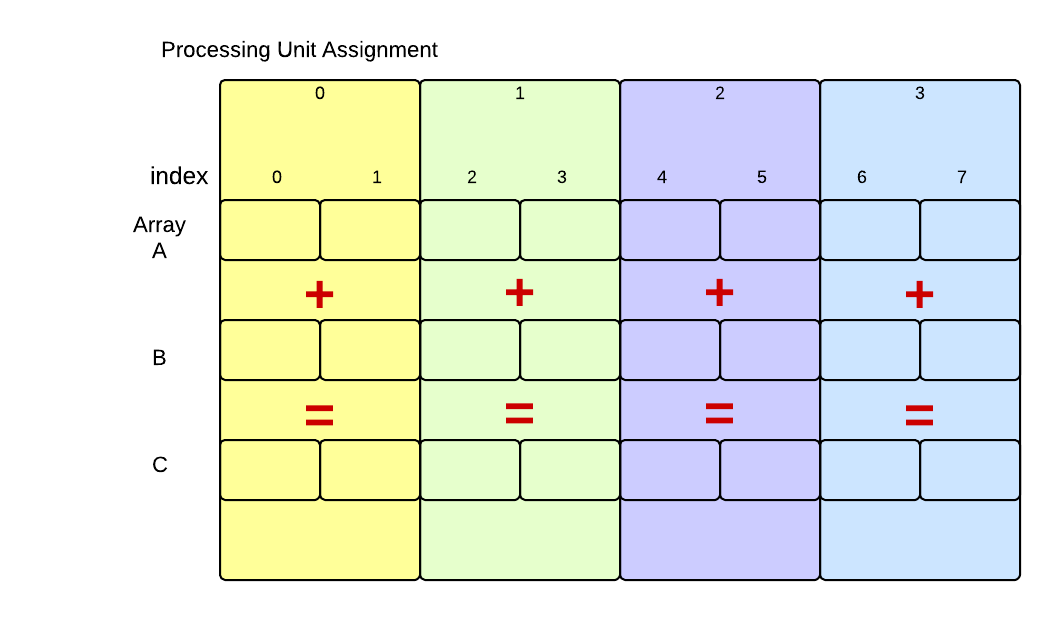
\includegraphics{Decomposition.png}
\end{figure}

Here we see our original problem with eight elements in each array. Processing unit 0 would work on the first two elements, processing unit 1 would work on the next two, and so on.  Theoretically, using four processing units executing concurrently, the work should get done in one-fourth the time it takes to run it sequentially.  In practice, this never quite happens, because of the overhead to start processing units and possible contention for resources, such as the arrays themselves.

For many larger problems with more sophisticated computations, however, this type of decomposition of computational tasks on data elements is very common and can speed up your program.  There is no standard terminology for this version of data decomposition; we like to refer to it as \emph{decomposing into equal-sized chunks}.  There are other possible types of decomposition and mapping of processing units to elements (perhaps others have been running through your mind). We limit ourselves to this particular way of decomposing, because:
\begin{itemize}
\item {} 
it occurs quite often,

\item {} 
it is a good way to do it in many situations because elements are stored contiguously in memory, and

\item {} 
you can concentrate on and learn one way of using multiple processing units.

\end{itemize}

Next we will examine example code for three combinations of parallel software and hardware:
\begin{itemize}
\item {} 
Message passing using the MPI library, which can be used on a cluster or a single multicore computer.

\item {} 
Shared memory and threads using the OpenMP compiler directives in gcc, which can be used on a multicore computer.

\item {} 
CUDA programming with the nvcc compiler, which can be used on a machine with a Graphics Procesing Unit, or GPU.

\end{itemize}


\chapter{Vector Add with MPI}
\label{Decomposition/MPI_VecAdd:vector-add-with-mpi}\label{Decomposition/MPI_VecAdd::doc}
Message passing is one way of distributing work to multiple \emph{processes} that run indepentdently and concurrently on either a single computer or a cluster of computers. The processes, which are designated to start up in the software and are run by the operating system of the computer, serve as the processing units. This type of parallel programming has been used for quite some time and the software libraries that make it available follow a standard called Message Passing Interface, or MPI.

One feature of MPI programming is that one single program designates what all the various processes will do-- a single program runs on all the processes. Each process has a number or \emph{rank}, and the value of the rank is used in the code to determine what each process will do.  In the following code, the process numbered 0 does some additional work that the other processes do not do. This is very common in message passing solutions, and process 0 is often referred to as the master, and the other processes are the workers.  In the code below, look for three places where a block of code starts with this line:

\begin{Verbatim}[commandchars=\\\{\}]
\PYG{k}{if} \PYG{p}{(}\PYG{n}{rank} \PYG{o}{=}\PYG{o}{=} \PYG{n}{MASTER}\PYG{p}{)}  \PYG{p}{\PYGZob{}}
\end{Verbatim}

This is where the master is doing special work that only needs to be done once by one process. In this case, it is the initialization of the arrays at the beginning of the computation, the check to ensure accuracy after the main computation of vector addition is completed, and freeing the memory for the arrays at the end.

The MPI syntax in this code takes some getting used to, but you should see the pattern of how the data decomposition is occuring for a process running this code:
\begin{enumerate}
\item {} 
First initialize your set of processes (the number of processes in designated when you run the code).

\item {} 
Determine how many processes there are working on the problem.

\item {} 
Determine which process rank I have.

\item {} 
If I am the master, initialze the data arrays.

\item {} 
Create smaller arrays for my portion of the work.

\item {} 
Scatter the equal-sized chunks of the larger original arrays from the master out to each process to work on.

\item {} 
Compute the vector addition on my chunk of data.

\item {} 
Gather the completed chunks of my array C and those of each process back onto the larger array on the master.

\item {} 
Terminate all the processes.

\end{enumerate}

The following code contains comments with these numbered steps where they occur.  This is the file
\textbf{VectorAdd/MPI/VA-MPI-simple.c} in the compressed tar file of examples that accompanies this reading.

\begin{Verbatim}[commandchars=\\\{\},numbers=left,firstnumber=1,stepnumber=1]
\PYG{c+cm}{/*}
\PYG{c+cm}{ *  Prerequisties:}
\PYG{c+cm}{ *     This code runs using an MPI library, either OpenMPI or MPICH2.}
\PYG{c+cm}{ *     These libraries can be installed in either a cluster of computers}
\PYG{c+cm}{ *     or a multicore machine.}
\PYG{c+cm}{ *     }
\PYG{c+cm}{ *  How to compile:}
\PYG{c+cm}{ *     mpicc -o vec-add VA-MPI-simple.c}
\PYG{c+cm}{ *}
\PYG{c+cm}{ *  How to execute:}
\PYG{c+cm}{ *     mpirun -np 2 ./vec-add}
\PYG{c+cm}{ *}
\PYG{c+cm}{ *     Note that this executes the code on 2 processes, using the -np command line flag.}
\PYG{c+cm}{ *     See ideas for further exploration of MPI using this code at the end of this file.}
\PYG{c+cm}{ */}


\PYG{c+cp}{\PYGZsh{}}\PYG{c+cp}{include "mpi.h"      }\PYG{c+c1}{// must have a system with an MPI library}
\PYG{c+cp}{\PYGZsh{}}\PYG{c+cp}{include \PYGZlt{}stdio.h\PYGZgt{}    }\PYG{c+c1}{//printf}
\PYG{c+cp}{\PYGZsh{}}\PYG{c+cp}{include \PYGZlt{}stdlib.h\PYGZgt{}   }\PYG{c+c1}{//malloc}

\PYG{c+cm}{/*}
\PYG{c+cm}{ * Definitions}
\PYG{c+cm}{ */}
\PYG{c+cp}{\PYGZsh{}}\PYG{c+cp}{define MASTER 0         }\PYG{c+c1}{//One process will take care of initialization}
\PYG{c+cp}{\PYGZsh{}}\PYG{c+cp}{define ARRAY\PYGZus{}SIZE 8     }\PYG{c+c1}{//Size of arrays that will be added together.}

\PYG{c+cm}{/*}
\PYG{c+cm}{ *  In MPI programs, the main function for the program is run on every}
\PYG{c+cm}{ *  process that gets initialized when you start up this code using mpirun.}
\PYG{c+cm}{ */}
\PYG{k+kt}{int} \PYG{n+nf}{main} \PYG{p}{(}\PYG{k+kt}{int} \PYG{n}{argc}\PYG{p}{,} \PYG{k+kt}{char} \PYG{o}{*}\PYG{n}{argv}\PYG{p}{[}\PYG{p}{]}\PYG{p}{)} 
\PYG{p}{\PYGZob{}}
	\PYG{c+c1}{// elements of arrays a and b will be added}
	\PYG{c+c1}{// and placed in array c}
	\PYG{k+kt}{int} \PYG{o}{*} \PYG{n}{a}\PYG{p}{;}
	\PYG{k+kt}{int} \PYG{o}{*} \PYG{n}{b}\PYG{p}{;} 
	\PYG{k+kt}{int} \PYG{o}{*} \PYG{n}{c}\PYG{p}{;}
	
	\PYG{k+kt}{int} \PYG{n}{total\PYGZus{}proc}\PYG{p}{;}	 \PYG{c+c1}{// total nuber of processes	}
	\PYG{k+kt}{int} \PYG{n}{rank}\PYG{p}{;}        \PYG{c+c1}{// rank of each process}
	\PYG{k+kt}{int} \PYG{n}{n\PYGZus{}per\PYGZus{}proc}\PYG{p}{;}	\PYG{c+c1}{// elements per process	}
	\PYG{k+kt}{int} \PYG{n}{n} \PYG{o}{=} \PYG{n}{ARRAY\PYGZus{}SIZE}\PYG{p}{;}   \PYG{c+c1}{// number of array elements}
	\PYG{k+kt}{int} \PYG{n}{i}\PYG{p}{;}       \PYG{c+c1}{// loop index}
		
	\PYG{n}{MPI\PYGZus{}Status} \PYG{n}{status}\PYG{p}{;}   \PYG{c+c1}{// not used in this arguably poor example}
	                     \PYG{c+c1}{// that is devoid of error checking.}

	\PYG{c+c1}{// 1. Initialization of MPI environment}
	\PYG{n}{MPI\PYGZus{}Init} \PYG{p}{(}\PYG{o}{\PYGZam{}}\PYG{n}{argc}\PYG{p}{,} \PYG{o}{\PYGZam{}}\PYG{n}{argv}\PYG{p}{)}\PYG{p}{;}
	\PYG{n}{MPI\PYGZus{}Comm\PYGZus{}size} \PYG{p}{(}\PYG{n}{MPI\PYGZus{}COMM\PYGZus{}WORLD}\PYG{p}{,} \PYG{o}{\PYGZam{}}\PYG{n}{total\PYGZus{}proc}\PYG{p}{)}\PYG{p}{;}
	\PYG{c+c1}{// 2. Now you know the total number of processes running in parallel}
	\PYG{n}{MPI\PYGZus{}Comm\PYGZus{}rank} \PYG{p}{(}\PYG{n}{MPI\PYGZus{}COMM\PYGZus{}WORLD}\PYG{p}{,}\PYG{o}{\PYGZam{}}\PYG{n}{rank}\PYG{p}{)}\PYG{p}{;}
	\PYG{c+c1}{// 3. Now you know the rank of the current process}
	
	\PYG{c+c1}{// Smaller arrays that will be held on each separate process}
    	\PYG{k+kt}{int} \PYG{o}{*} \PYG{n}{ap}\PYG{p}{;}
	\PYG{k+kt}{int} \PYG{o}{*} \PYG{n}{bp}\PYG{p}{;}
	\PYG{k+kt}{int} \PYG{o}{*} \PYG{n}{cp}\PYG{p}{;}
	
	\PYG{c+c1}{// 4. We choose process rank 0 to be the root, or master,}
	\PYG{c+c1}{// which will be used to  initialize the full arrays.}
	\PYG{k}{if} \PYG{p}{(}\PYG{n}{rank} \PYG{o}{=}\PYG{o}{=} \PYG{n}{MASTER}\PYG{p}{)}  \PYG{p}{\PYGZob{}}
		\PYG{n}{a} \PYG{o}{=} \PYG{p}{(}\PYG{k+kt}{int} \PYG{o}{*}\PYG{p}{)} \PYG{n}{malloc}\PYG{p}{(}\PYG{k}{sizeof}\PYG{p}{(}\PYG{k+kt}{int}\PYG{p}{)}\PYG{o}{*}\PYG{n}{n}\PYG{p}{)}\PYG{p}{;}
		\PYG{n}{b} \PYG{o}{=} \PYG{p}{(}\PYG{k+kt}{int} \PYG{o}{*}\PYG{p}{)} \PYG{n}{malloc}\PYG{p}{(}\PYG{k}{sizeof}\PYG{p}{(}\PYG{k+kt}{int}\PYG{p}{)}\PYG{o}{*}\PYG{n}{n}\PYG{p}{)}\PYG{p}{;}
		\PYG{n}{c} \PYG{o}{=} \PYG{p}{(}\PYG{k+kt}{int} \PYG{o}{*}\PYG{p}{)} \PYG{n}{malloc}\PYG{p}{(}\PYG{k}{sizeof}\PYG{p}{(}\PYG{k+kt}{int}\PYG{p}{)}\PYG{o}{*}\PYG{n}{n}\PYG{p}{)}\PYG{p}{;}
		
		\PYG{c+c1}{// initialize arrays a and b with consecutive integer values}
		\PYG{c+c1}{// as a simple example}
		\PYG{k}{for}\PYG{p}{(}\PYG{n}{i}\PYG{o}{=}\PYG{l+m+mi}{0}\PYG{p}{;}\PYG{n}{i}\PYG{o}{\PYGZlt{}}\PYG{n}{n}\PYG{p}{;}\PYG{n}{i}\PYG{o}{+}\PYG{o}{+}\PYG{p}{)}
			\PYG{n}{a}\PYG{p}{[}\PYG{n}{i}\PYG{p}{]} \PYG{o}{=} \PYG{n}{i}\PYG{p}{;}
		\PYG{k}{for}\PYG{p}{(}\PYG{n}{i}\PYG{o}{=}\PYG{l+m+mi}{0}\PYG{p}{;}\PYG{n}{i}\PYG{o}{\PYGZlt{}}\PYG{n}{n}\PYG{p}{;}\PYG{n}{i}\PYG{o}{+}\PYG{o}{+}\PYG{p}{)}
			\PYG{n}{b}\PYG{p}{[}\PYG{n}{i}\PYG{p}{]} \PYG{o}{=} \PYG{n}{i}\PYG{p}{;}
	\PYG{p}{\PYGZcb{}}
	
	\PYG{c+c1}{// All processes take part in the calculations concurrently}
		
	\PYG{c+c1}{// determine how many elements each process will work on}
	\PYG{n}{n\PYGZus{}per\PYGZus{}proc} \PYG{o}{=} \PYG{n}{n}\PYG{o}{/}\PYG{n}{total\PYGZus{}proc}\PYG{p}{;}
	\PYG{c+c1}{/////// NOTE:}
	\PYG{c+c1}{// In this simple version, the number of processes needs to}
	\PYG{c+c1}{// divide evenly into the number of elements in the array}
	\PYG{c+c1}{///////////}
	
	\PYG{c+c1}{// 5. Initialize my smaller subsections of the larger array}
	\PYG{n}{ap} \PYG{o}{=} \PYG{p}{(}\PYG{k+kt}{int} \PYG{o}{*}\PYG{p}{)} \PYG{n}{malloc}\PYG{p}{(}\PYG{k}{sizeof}\PYG{p}{(}\PYG{k+kt}{int}\PYG{p}{)}\PYG{o}{*}\PYG{n}{n\PYGZus{}per\PYGZus{}proc}\PYG{p}{)}\PYG{p}{;}
	\PYG{n}{bp} \PYG{o}{=} \PYG{p}{(}\PYG{k+kt}{int} \PYG{o}{*}\PYG{p}{)} \PYG{n}{malloc}\PYG{p}{(}\PYG{k}{sizeof}\PYG{p}{(}\PYG{k+kt}{int}\PYG{p}{)}\PYG{o}{*}\PYG{n}{n\PYGZus{}per\PYGZus{}proc}\PYG{p}{)}\PYG{p}{;}
	\PYG{n}{cp} \PYG{o}{=} \PYG{p}{(}\PYG{k+kt}{int} \PYG{o}{*}\PYG{p}{)} \PYG{n}{malloc}\PYG{p}{(}\PYG{k}{sizeof}\PYG{p}{(}\PYG{k+kt}{int}\PYG{p}{)}\PYG{o}{*}\PYG{n}{n\PYGZus{}per\PYGZus{}proc}\PYG{p}{)}\PYG{p}{;}
	
	\PYG{c+c1}{// 6.}
	\PYG{c+c1}{//scattering array a from MASTER node out to the other nodes}
	\PYG{n}{MPI\PYGZus{}Scatter}\PYG{p}{(}\PYG{n}{a}\PYG{p}{,} \PYG{n}{n\PYGZus{}per\PYGZus{}proc}\PYG{p}{,} \PYG{n}{MPI\PYGZus{}INT}\PYG{p}{,} \PYG{n}{ap}\PYG{p}{,} \PYG{n}{n\PYGZus{}per\PYGZus{}proc}\PYG{p}{,} \PYG{n}{MPI\PYGZus{}INT}\PYG{p}{,} \PYG{n}{MASTER}\PYG{p}{,} \PYG{n}{MPI\PYGZus{}COMM\PYGZus{}WORLD}\PYG{p}{)}\PYG{p}{;} 
	\PYG{c+c1}{//scattering array b from MASTER node out to the other node}
	\PYG{n}{MPI\PYGZus{}Scatter}\PYG{p}{(}\PYG{n}{b}\PYG{p}{,} \PYG{n}{n\PYGZus{}per\PYGZus{}proc}\PYG{p}{,} \PYG{n}{MPI\PYGZus{}INT}\PYG{p}{,} \PYG{n}{bp}\PYG{p}{,} \PYG{n}{n\PYGZus{}per\PYGZus{}proc}\PYG{p}{,} \PYG{n}{MPI\PYGZus{}INT}\PYG{p}{,} \PYG{n}{MASTER}\PYG{p}{,} \PYG{n}{MPI\PYGZus{}COMM\PYGZus{}WORLD}\PYG{p}{)}\PYG{p}{;} 
	
	\PYG{c+c1}{// 7. Compute the addition of elements in my subsection of the array}
	\PYG{k}{for}\PYG{p}{(}\PYG{n}{i}\PYG{o}{=}\PYG{l+m+mi}{0}\PYG{p}{;}\PYG{n}{i}\PYG{o}{\PYGZlt{}}\PYG{n}{n\PYGZus{}per\PYGZus{}proc}\PYG{p}{;}\PYG{n}{i}\PYG{o}{+}\PYG{o}{+}\PYG{p}{)}
		\PYG{n}{cp}\PYG{p}{[}\PYG{n}{i}\PYG{p}{]} \PYG{o}{=} \PYG{n}{ap}\PYG{p}{[}\PYG{n}{i}\PYG{p}{]}\PYG{o}{+}\PYG{n}{bp}\PYG{p}{[}\PYG{n}{i}\PYG{p}{]}\PYG{p}{;}
	
	\PYG{c+c1}{// 8. MASTER node gathering array c from the workers}
	\PYG{n}{MPI\PYGZus{}Gather}\PYG{p}{(}\PYG{n}{cp}\PYG{p}{,} \PYG{n}{n\PYGZus{}per\PYGZus{}proc}\PYG{p}{,} \PYG{n}{MPI\PYGZus{}INT}\PYG{p}{,} \PYG{n}{c}\PYG{p}{,} \PYG{n}{n\PYGZus{}per\PYGZus{}proc}\PYG{p}{,} \PYG{n}{MPI\PYGZus{}INT}\PYG{p}{,} \PYG{n}{MASTER}\PYG{p}{,} \PYG{n}{MPI\PYGZus{}COMM\PYGZus{}WORLD}\PYG{p}{)}\PYG{p}{;}

\PYG{c+c1}{/////////////////////// all concurrent processes are finished once they all communicate}
\PYG{c+c1}{/////////////////////// data back to the master via the gather function.}

	\PYG{c+c1}{// Master process gets to here only when it has been able to gather from all processes}
	\PYG{k}{if} \PYG{p}{(}\PYG{n}{rank} \PYG{o}{=}\PYG{o}{=} \PYG{n}{MASTER}\PYG{p}{)}  \PYG{p}{\PYGZob{}}			
		\PYG{c+c1}{// sanity check the result  (a test we would eventually leave out)}
		\PYG{k+kt}{int} \PYG{n}{good} \PYG{o}{=} \PYG{l+m+mi}{1}\PYG{p}{;}
		\PYG{k}{for}\PYG{p}{(}\PYG{n}{i}\PYG{o}{=}\PYG{l+m+mi}{0}\PYG{p}{;}\PYG{n}{i}\PYG{o}{\PYGZlt{}}\PYG{n}{n}\PYG{p}{;}\PYG{n}{i}\PYG{o}{+}\PYG{o}{+}\PYG{p}{)} \PYG{p}{\PYGZob{}}
			\PYG{c+c1}{//printf ("\PYGZpc{}d ", c[i]);}
			\PYG{k}{if} \PYG{p}{(}\PYG{n}{c}\PYG{p}{[}\PYG{n}{i}\PYG{p}{]} \PYG{o}{!}\PYG{o}{=} \PYG{n}{a}\PYG{p}{[}\PYG{n}{i}\PYG{p}{]} \PYG{o}{+} \PYG{n}{b}\PYG{p}{[}\PYG{n}{i}\PYG{p}{]}\PYG{p}{)} \PYG{p}{\PYGZob{}}
				\PYG{n}{printf}\PYG{p}{(}\PYG{l+s}{"}\PYG{l+s}{problem at index \PYGZpc{}lld}\PYG{l+s+se}{\PYGZbs{}n}\PYG{l+s}{"}\PYG{p}{,} \PYG{n}{i}\PYG{p}{)}\PYG{p}{;}
				\PYG{n}{good} \PYG{o}{=} \PYG{l+m+mi}{0}\PYG{p}{;}
				\PYG{k}{break}\PYG{p}{;}
			\PYG{p}{\PYGZcb{}}
		\PYG{p}{\PYGZcb{}}
		\PYG{k}{if} \PYG{p}{(}\PYG{n}{good}\PYG{p}{)} \PYG{p}{\PYGZob{}}
			\PYG{n}{printf} \PYG{p}{(}\PYG{l+s}{"}\PYG{l+s}{Values correct!}\PYG{l+s+se}{\PYGZbs{}n}\PYG{l+s}{"}\PYG{p}{)}\PYG{p}{;}
		\PYG{p}{\PYGZcb{}}
		
	\PYG{p}{\PYGZcb{}}

	\PYG{c+c1}{// clean up memory}
	\PYG{k}{if} \PYG{p}{(}\PYG{n}{rank} \PYG{o}{=}\PYG{o}{=} \PYG{n}{MASTER}\PYG{p}{)}  \PYG{p}{\PYGZob{}}
		\PYG{n}{free}\PYG{p}{(}\PYG{n}{a}\PYG{p}{)}\PYG{p}{;}  \PYG{n}{free}\PYG{p}{(}\PYG{n}{b}\PYG{p}{)}\PYG{p}{;} \PYG{n}{free}\PYG{p}{(}\PYG{n}{c}\PYG{p}{)}\PYG{p}{;}
	\PYG{p}{\PYGZcb{}}
	\PYG{n}{free}\PYG{p}{(}\PYG{n}{ap}\PYG{p}{)}\PYG{p}{;}  \PYG{n}{free}\PYG{p}{(}\PYG{n}{bp}\PYG{p}{)}\PYG{p}{;} \PYG{n}{free}\PYG{p}{(}\PYG{n}{cp}\PYG{p}{)}\PYG{p}{;}
	
	\PYG{c+c1}{// 9. Terminate MPI Environment and Processes}
	\PYG{n}{MPI\PYGZus{}Finalize}\PYG{p}{(}\PYG{p}{)}\PYG{p}{;}  
	
	\PYG{k}{return} \PYG{l+m+mi}{0}\PYG{p}{;}
\PYG{p}{\PYGZcb{}}
\end{Verbatim}


\chapter{Vector Add with OpenMP}
\label{Decomposition/OpenMP_VecAdd:vector-add-with-openmp}\label{Decomposition/OpenMP_VecAdd::doc}
Computers with multicore processors and a single shared memory space are the norm, including not only laptops and desktops, but also most phones and tablets. Using multiple cores concurrently on these machines, can be done in several programming languages; we will demonstrate the use of C with a set of compiler directives and library functions known as OpenMP.  The OpenMP standard is built into many C compilers, including gcc on unix machines.

OpenMP on shared memory multicore machines creates \emph{threads} that execute concurrently.  The creation of these threads is implicit and built by the compiler when you insert special directives in the C code called \emph{pragmas}.
The code that begins executing main() is considered thread 0. At certain points in the code, you can designate that more threads should be used in parallel and exucute concurrently. This is called \emph{forking} threads.

In the code below, you will see this pragma, which is implicitly forking the threads to complete the computation on equal chunks of the orginal array:

\begin{Verbatim}[commandchars=\\\{\}]
\PYG{c+cp}{\PYGZsh{}}\PYG{c+cp}{pragma omp parallel for shared(a, b, c) private(i) schedule(static, 2)}
\end{Verbatim}

The \code{shared} keyword indicates that the arrays are shared in the same memory space for all threads, and the \code{private} keyword indicates that each thread will have its own copy of the index counter i that it will increment.

The \code{schedule} keyword is used in this pragma to indicate how many consecutive iterations of the loop, and thus computations on consecutive elements of the arrays, that each thread will execute.  In data decomposition, we like to call this the \textbf{chunk size} assigned to each thread (not necessarily a universal term, but  hopefully it conveys the idea). To mimic our simple 8-element example, this code (shown below) sets the number of threads to 4 and the chunk size to 2.

The syntax of this OpenMP code example below is very similar to the original sequential version. In fact, it was derived from the sequential version by adding this pragma, including the OpenMP library, called omp.h, setting how many threads to use and the chuck size just before the forking, and adding some print statements to illustrate the decomposition and verify the results.

This pragma around for loops is built into openMP because this `repeat N times'' pattern occurs so frequently in a great deal of code. This simplicity can be deceiving, however-- this particular example lends itself well to having the threads share data, but other types of problems are not this simple.  This type of data decomposition example is sometimes called \emph{embarassingly parallel}, because each thread can read and update data that no other thread should ever touch.

This code is the file
\textbf{VectorAdd/OpenMP/VA-OMP-simple.c} in the compressed tar file of examples that accompanies this reading.

\begin{Verbatim}[commandchars=\\\{\},numbers=left,firstnumber=1,stepnumber=1]
\PYG{c+cp}{\PYGZsh{}}\PYG{c+cp}{include \PYGZlt{}stdlib.h\PYGZgt{}   }\PYG{c+c1}{//malloc and free}
\PYG{c+cp}{\PYGZsh{}}\PYG{c+cp}{include \PYGZlt{}stdio.h\PYGZgt{}    }\PYG{c+c1}{//printf}
\PYG{c+cp}{\PYGZsh{}}\PYG{c+cp}{include \PYGZlt{}omp.h\PYGZgt{}      }\PYG{c+c1}{//OpenMP}

\PYG{c+c1}{// Very small values for this simple illustrative example}
\PYG{c+cp}{\PYGZsh{}}\PYG{c+cp}{define ARRAY\PYGZus{}SIZE 8     }\PYG{c+c1}{//Size of arrays whose elements will be added together.}
\PYG{c+cp}{\PYGZsh{}}\PYG{c+cp}{define NUM\PYGZus{}THREADS 4    }\PYG{c+c1}{//Number of threads to use for vector addition.}

\PYG{c+cm}{/*}
\PYG{c+cm}{ *  Classic vector addition using openMP default data decomposition.}
\PYG{c+cm}{ *}
\PYG{c+cm}{ *  Compile using gcc like this:}
\PYG{c+cm}{ *  	gcc -o va-omp-simple VA-OMP-simple.c -fopenmp}
\PYG{c+cm}{ *}
\PYG{c+cm}{ *  Execute:}
\PYG{c+cm}{ *  	./va-omp-simple}
\PYG{c+cm}{ */}
\PYG{k+kt}{int} \PYG{n+nf}{main} \PYG{p}{(}\PYG{k+kt}{int} \PYG{n}{argc}\PYG{p}{,} \PYG{k+kt}{char} \PYG{o}{*}\PYG{n}{argv}\PYG{p}{[}\PYG{p}{]}\PYG{p}{)} 
\PYG{p}{\PYGZob{}}
	\PYG{c+c1}{// elements of arrays a and b will be added}
	\PYG{c+c1}{// and placed in array c}
	\PYG{k+kt}{int} \PYG{o}{*} \PYG{n}{a}\PYG{p}{;}
	\PYG{k+kt}{int} \PYG{o}{*} \PYG{n}{b}\PYG{p}{;} 
	\PYG{k+kt}{int} \PYG{o}{*} \PYG{n}{c}\PYG{p}{;}
        
        \PYG{k+kt}{int} \PYG{n}{n} \PYG{o}{=} \PYG{n}{ARRAY\PYGZus{}SIZE}\PYG{p}{;}                 \PYG{c+c1}{// number of array elements}
	\PYG{k+kt}{int} \PYG{n}{n\PYGZus{}per\PYGZus{}thread}\PYG{p}{;}                   \PYG{c+c1}{// elements per thread}
	\PYG{k+kt}{int} \PYG{n}{total\PYGZus{}threads} \PYG{o}{=} \PYG{n}{NUM\PYGZus{}THREADS}\PYG{p}{;}    \PYG{c+c1}{// number of threads to use  }
	\PYG{k+kt}{int} \PYG{n}{i}\PYG{p}{;}       \PYG{c+c1}{// loop index}
        
        \PYG{c+c1}{// allocate spce for the arrays}
        \PYG{n}{a} \PYG{o}{=} \PYG{p}{(}\PYG{k+kt}{int} \PYG{o}{*}\PYG{p}{)} \PYG{n}{malloc}\PYG{p}{(}\PYG{k}{sizeof}\PYG{p}{(}\PYG{k+kt}{int}\PYG{p}{)}\PYG{o}{*}\PYG{n}{n}\PYG{p}{)}\PYG{p}{;}
	\PYG{n}{b} \PYG{o}{=} \PYG{p}{(}\PYG{k+kt}{int} \PYG{o}{*}\PYG{p}{)} \PYG{n}{malloc}\PYG{p}{(}\PYG{k}{sizeof}\PYG{p}{(}\PYG{k+kt}{int}\PYG{p}{)}\PYG{o}{*}\PYG{n}{n}\PYG{p}{)}\PYG{p}{;}
	\PYG{n}{c} \PYG{o}{=} \PYG{p}{(}\PYG{k+kt}{int} \PYG{o}{*}\PYG{p}{)} \PYG{n}{malloc}\PYG{p}{(}\PYG{k}{sizeof}\PYG{p}{(}\PYG{k+kt}{int}\PYG{p}{)}\PYG{o}{*}\PYG{n}{n}\PYG{p}{)}\PYG{p}{;}

        \PYG{c+c1}{// initialize arrays a and b with consecutive integer values}
	\PYG{c+c1}{// as a simple example}
        \PYG{k}{for}\PYG{p}{(}\PYG{n}{i}\PYG{o}{=}\PYG{l+m+mi}{0}\PYG{p}{;} \PYG{n}{i}\PYG{o}{\PYGZlt{}}\PYG{n}{n}\PYG{p}{;} \PYG{n}{i}\PYG{o}{+}\PYG{o}{+}\PYG{p}{)} \PYG{p}{\PYGZob{}}
            \PYG{n}{a}\PYG{p}{[}\PYG{n}{i}\PYG{p}{]} \PYG{o}{=} \PYG{n}{i}\PYG{p}{;}
        \PYG{p}{\PYGZcb{}}
        \PYG{k}{for}\PYG{p}{(}\PYG{n}{i}\PYG{o}{=}\PYG{l+m+mi}{0}\PYG{p}{;} \PYG{n}{i}\PYG{o}{\PYGZlt{}}\PYG{n}{n}\PYG{p}{;} \PYG{n}{i}\PYG{o}{+}\PYG{o}{+}\PYG{p}{)} \PYG{p}{\PYGZob{}}
            \PYG{n}{b}\PYG{p}{[}\PYG{n}{i}\PYG{p}{]} \PYG{o}{=} \PYG{n}{i}\PYG{p}{;}
        \PYG{p}{\PYGZcb{}}   
        
	\PYG{c+c1}{// Additional work to set the number of threads.}
	\PYG{c+c1}{// We hard-code to 4 for illustration purposes only.}
	\PYG{n}{omp\PYGZus{}set\PYGZus{}num\PYGZus{}threads}\PYG{p}{(}\PYG{n}{total\PYGZus{}threads}\PYG{p}{)}\PYG{p}{;}
	
	\PYG{c+c1}{// determine how many elements each process will work on}
	\PYG{n}{n\PYGZus{}per\PYGZus{}thread} \PYG{o}{=} \PYG{n}{n}\PYG{o}{/}\PYG{n}{total\PYGZus{}threads}\PYG{p}{;}
	
        \PYG{c+c1}{// Compute the vector addition}
	\PYG{c+c1}{// Here is where the 4 threads are specifically 'forked' to}
	\PYG{c+c1}{// execute in parallel. This is directed by the pragma and}
	\PYG{c+c1}{// thread forking is compiled into the resulting exacutable.}
	\PYG{c+c1}{// Here we use a 'static schedule' so each thread works on  }
	\PYG{c+c1}{// a 2-element chunk of the original 8-element arrays.}
	\PYG{c+cp}{\PYGZsh{}}\PYG{c+cp}{pragma omp parallel for shared(a, b, c) private(i) schedule(static, n\PYGZus{}per\PYGZus{}thread)}
        \PYG{k}{for}\PYG{p}{(}\PYG{n}{i}\PYG{o}{=}\PYG{l+m+mi}{0}\PYG{p}{;} \PYG{n}{i}\PYG{o}{\PYGZlt{}}\PYG{n}{n}\PYG{p}{;} \PYG{n}{i}\PYG{o}{+}\PYG{o}{+}\PYG{p}{)} \PYG{p}{\PYGZob{}}
		\PYG{n}{c}\PYG{p}{[}\PYG{n}{i}\PYG{p}{]} \PYG{o}{=} \PYG{n}{a}\PYG{p}{[}\PYG{n}{i}\PYG{p}{]}\PYG{o}{+}\PYG{n}{b}\PYG{p}{[}\PYG{n}{i}\PYG{p}{]}\PYG{p}{;}
		\PYG{c+c1}{// Which thread am I? Show who works on what for this samll example}
		\PYG{n}{printf}\PYG{p}{(}\PYG{l+s}{"}\PYG{l+s}{Thread \PYGZpc{}d works on element\PYGZpc{}d}\PYG{l+s+se}{\PYGZbs{}n}\PYG{l+s}{"}\PYG{p}{,} \PYG{n}{omp\PYGZus{}get\PYGZus{}thread\PYGZus{}num}\PYG{p}{(}\PYG{p}{)}\PYG{p}{,} \PYG{n}{i}\PYG{p}{)}\PYG{p}{;}
        \PYG{p}{\PYGZcb{}}
	
	\PYG{c+c1}{// Check for correctness (only plausible for small vector size)}
	\PYG{c+c1}{// A test we would eventually leave out}
	\PYG{n}{printf}\PYG{p}{(}\PYG{l+s}{"}\PYG{l+s}{i}\PYG{l+s+se}{\PYGZbs{}t}\PYG{l+s}{a[i]}\PYG{l+s+se}{\PYGZbs{}t}\PYG{l+s}{+}\PYG{l+s+se}{\PYGZbs{}t}\PYG{l+s}{b[i]}\PYG{l+s+se}{\PYGZbs{}t}\PYG{l+s}{=}\PYG{l+s+se}{\PYGZbs{}t}\PYG{l+s}{c[i]}\PYG{l+s+se}{\PYGZbs{}n}\PYG{l+s}{"}\PYG{p}{)}\PYG{p}{;}
        \PYG{k}{for}\PYG{p}{(}\PYG{n}{i}\PYG{o}{=}\PYG{l+m+mi}{0}\PYG{p}{;} \PYG{n}{i}\PYG{o}{\PYGZlt{}}\PYG{n}{n}\PYG{p}{;} \PYG{n}{i}\PYG{o}{+}\PYG{o}{+}\PYG{p}{)} \PYG{p}{\PYGZob{}}
		\PYG{n}{printf}\PYG{p}{(}\PYG{l+s}{"}\PYG{l+s}{\PYGZpc{}d}\PYG{l+s+se}{\PYGZbs{}t}\PYG{l+s}{\PYGZpc{}d}\PYG{l+s+se}{\PYGZbs{}t}\PYG{l+s+se}{\PYGZbs{}t}\PYG{l+s}{\PYGZpc{}d}\PYG{l+s+se}{\PYGZbs{}t}\PYG{l+s+se}{\PYGZbs{}t}\PYG{l+s}{\PYGZpc{}d}\PYG{l+s+se}{\PYGZbs{}n}\PYG{l+s}{"}\PYG{p}{,} \PYG{n}{i}\PYG{p}{,} \PYG{n}{a}\PYG{p}{[}\PYG{n}{i}\PYG{p}{]}\PYG{p}{,} \PYG{n}{b}\PYG{p}{[}\PYG{n}{i}\PYG{p}{]}\PYG{p}{,} \PYG{n}{c}\PYG{p}{[}\PYG{n}{i}\PYG{p}{]}\PYG{p}{)}\PYG{p}{;}
        \PYG{p}{\PYGZcb{}}
	
        \PYG{c+c1}{// clean up memory}
        \PYG{n}{free}\PYG{p}{(}\PYG{n}{a}\PYG{p}{)}\PYG{p}{;}  \PYG{n}{free}\PYG{p}{(}\PYG{n}{b}\PYG{p}{)}\PYG{p}{;} \PYG{n}{free}\PYG{p}{(}\PYG{n}{c}\PYG{p}{)}\PYG{p}{;}
	
	\PYG{k}{return} \PYG{l+m+mi}{0}\PYG{p}{;}
\PYG{p}{\PYGZcb{}}
\end{Verbatim}


\chapter{Vector Add with CUDA}
\label{Decomposition/CUDA_VecAdd:vector-add-with-cuda}\label{Decomposition/CUDA_VecAdd::doc}
Using the CUDA C language for general purpose computing on GPUs is well-suited to the vector addition problem, though there is a small amount of additional information you will need to make the code example clear.  On GPU co-processors, there are many more cores available than on traditional multicore CPUs. Each of these cores can execute a \emph{thread} of instructions indicated in the code. Unlike the threads and processes of OpenMP and MPI, CUDA adds extra layers of organization of the threads: programmers set up \emph{blocks} containing a certain number of threads, and organize the blocks into a \emph{grid}.

For the problem we originally posed, where we had 8 elements in an array, one possible organization we could define in CUDA would be 4 blocks of 2 threads each, like this:
\begin{figure}[htbp]
\centering

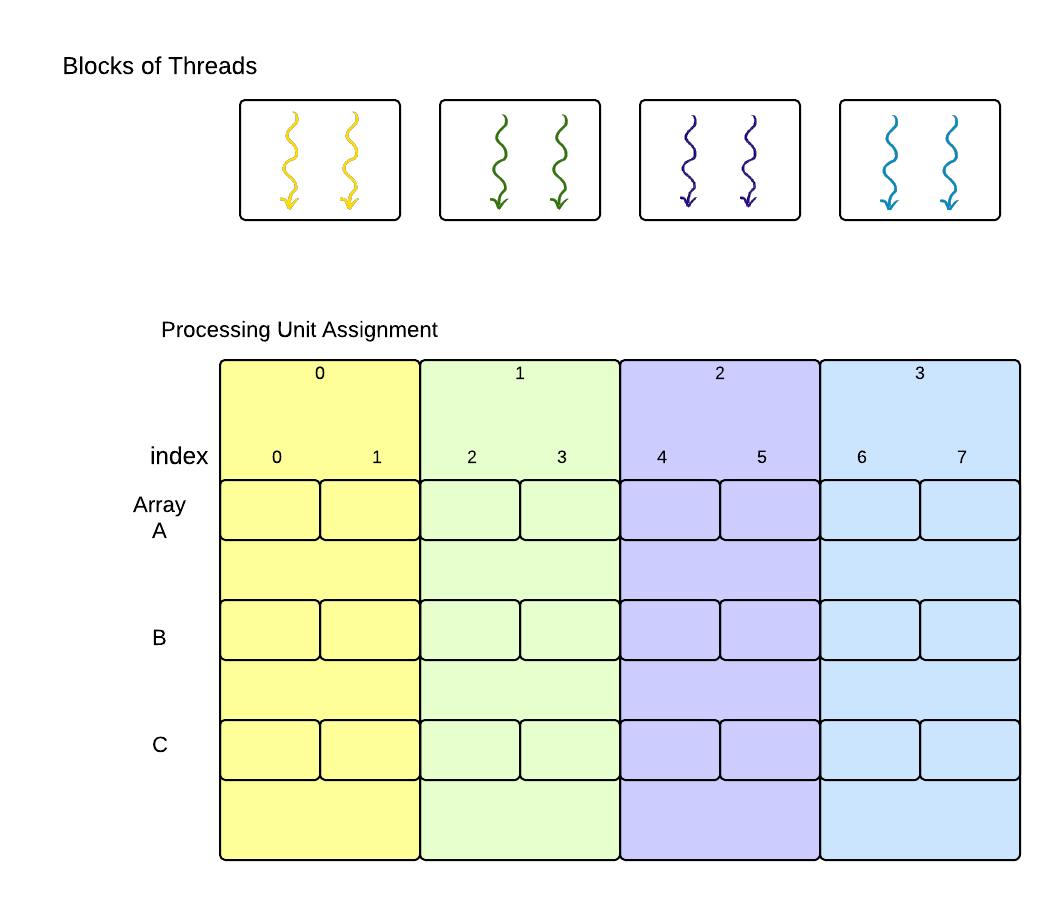
\includegraphics{CUDABlocksThreads.png}
\end{figure}

CUDA convention has been to depict treads as squiggly lines with arowheads, as shown above. In this case, the 4 blocks of threads that form the 1-dimensional grid become analogous to the processing units that we would assign to the portions of the array that would be run in parallel.  In contrast to OpenMP and MPI, however, the individual threads within the blocks would each work on one data element of the array \footnote{
Each GPU, depending on what type it is, can run a certain number of CUDA blocks containing some number of threads concurrently.  Your code can define the number of blocks and the number of threads per block, and the hardware will run as many as possible concurrently.  The maximum number of threads you can declare in a block is 1024, while the number of blocks you can declare is a very large number that depends on your GPU card.  Here we show a simple case of four blocks of 2 threads each, which in CUDA terminology forms a grid of blocks.  This particular grid of blocks would enable each element in an array of size 8 to be computed concurrently in parallel by 8 CUDA threads. To envision how the decomposition of the work might occur, imagine that the block of yellow threads corresponds to processing unit 0; similarly for each additional block of threads.
}.


\section{Determining the thread number}
\label{Decomposition/CUDA_VecAdd:determining-the-thread-number}
In all parallel programs that define one program that all threads will run, it is important to know which thread we are so that we can calculate what elements of the original array are assigned to us.  We saw with the MPI program, we could determine what the `rank' of the process was that was executing.  In the OpenMP example in the previous section, thread number assignment to sections of the array in the for loop was implicit \footnote{
This isn't always the case in OpenMP programs-- you can know just what you are and execute a section of code accordingly.
}.
In CUDA programs, we always determine which thread is running and use that to determine what portion of data to work on. The mapping of work is up to the programmer.

In CUDA programs, we set up the number of blocks that form the grid and we define how many threads will be used in each block. Once these are set, we have access to variables supplied by the CUDA library that help us define just what thread is executing. The following diagram shows how three of the available variables, corresponding to the grid, blocks, and threads within the blocks would be assigned for our above example decomposition:
\begin{figure}[htbp]
\centering

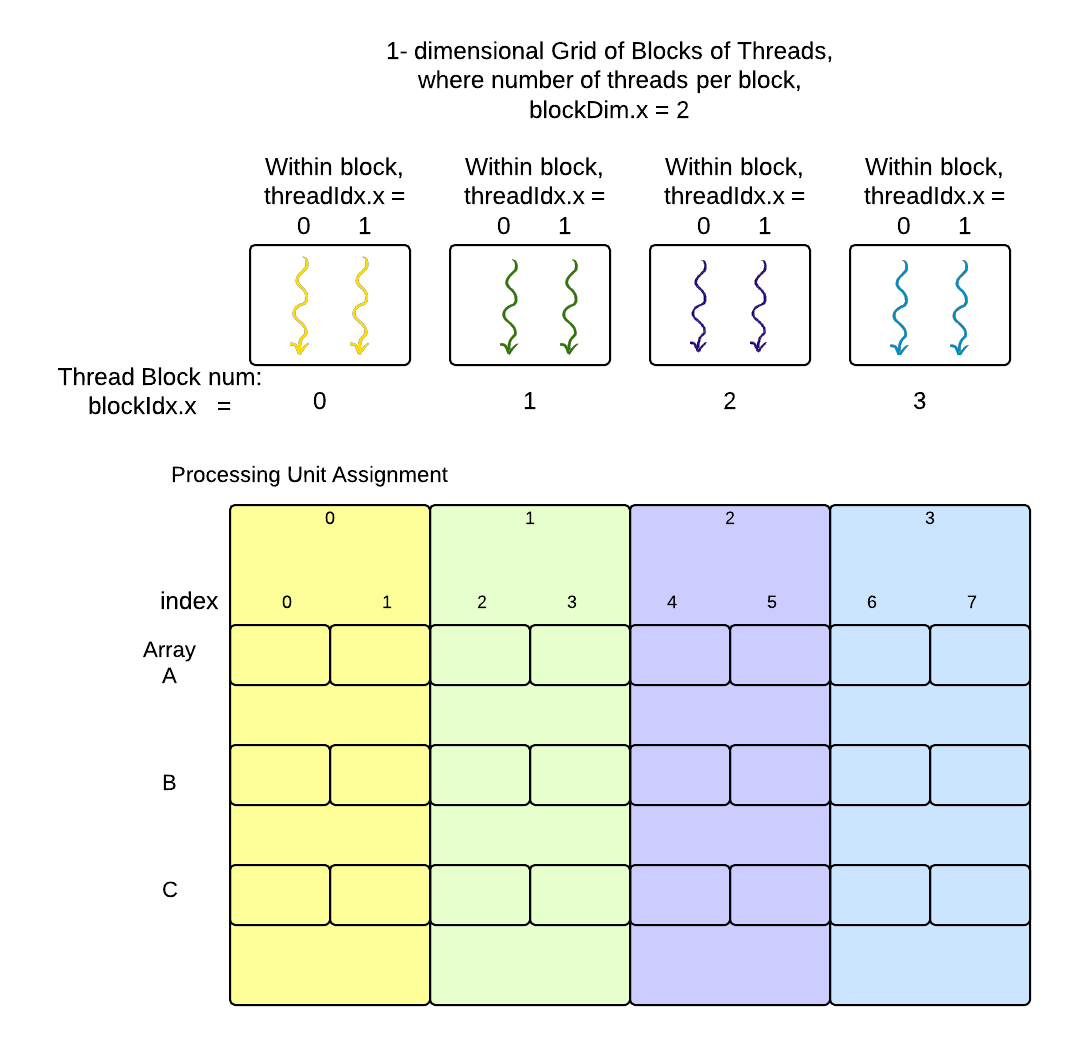
\includegraphics{CUDABThreadNumCalc.png}
\end{figure}

In this case of 1-dimensional arrays whose elements are being added, it is intuative to use a 1-dimensional grid of blocks, each of which has a 1-dimensional set of threads within it. For more complicated data, CUDA does let us define two or three-dimensional groupings of blocks and threads, but we will concentrate one this 1-dimensional example here.  In this case, we will use the `x' dimension provided by CUDA variables (the `y' and `z' dimensions are available for the complex cases when our data would naturally map to them). The three variables that we can access in CUDA code for this example shown above are:
\begin{enumerate}
\item {} 
\code{threadIdx.x} represents a thread's index along the x dimension within the block.

\item {} 
\code{blockIdx.x} represents a thread's block's index along the x dimension within the grid.

\item {} 
\code{blockDim.x} represents the number of threads per block in the x direction.

\end{enumerate}

In our simple example, there are a total of eight threads executing, each one numbered from 0 through 7. Each thread executing code on the GPU can determine which thread it is by using the above variables like this:

\begin{Verbatim}[commandchars=\\\{\}]
\PYG{k+kt}{int} \PYG{n}{tid} \PYG{o}{=} \PYG{n}{blockDim}\PYG{p}{.}\PYG{n}{x} \PYG{o}{*} \PYG{n}{blockIdx}\PYG{p}{.}\PYG{n}{x} \PYG{o}{+} \PYG{n}{threadIdx}\PYG{p}{.}\PYG{n}{x}\PYG{p}{;}
\end{Verbatim}


\section{The Host and the Device}
\label{Decomposition/CUDA_VecAdd:the-host-and-the-device}
CUDA programs execute code on a GPU, which is a co-processor, because it is a device on a card that is separate from the motherboard holding the CPU, or central processing unit.  In CUDA programming, the primary motherboard with the CPU is referred to as the \emph{host} and the GPU co-processor is usually called the \emph{device}.  The GPU device has separate memory and different circuitry for executing instructions. Code to be executed on the GPU must be compiled for its instrution set.


\section{CUDA Code for Vector Add}
\label{Decomposition/CUDA_VecAdd:cuda-code-for-vector-add}
The overall structure of a CUDA program that uses the GPU for computation is as follows:
\begin{enumerate}
\item {} 
Define the the code that will run on the device in a separate function, called the \emph{kernel} function.

\item {} \begin{description}
\item[{In the main program running on the host's CPU:}] \leavevmode\begin{enumerate}
\item {} 
allocate memory on the host for the data arrays.

\item {} 
initialze the data arrays in the host's memory.

\item {} 
allocate separate memory on the GPU device for the data arrays.

\item {} 
copy data arrays from the host memory to the GPU device memory.

\end{enumerate}

\end{description}

\item {} 
On the GPU device, execute the \emph{kernel} function that computes new data values given the original arrays. Specify how many blocks and threads per block to use for this computation.

\item {} 
After the \emph{kernel} function completes, copy the computed values from the GPU device memory back to the host's memory.

\end{enumerate}

Here is the actual code example for 8-element vector addition, with these above steps numbered. This is in the file
\textbf{VectorAdd/CUDA/VA-GPU-simple.cu} in the compressed tar file of examples that accompanies this reading.

\begin{Verbatim}[commandchars=\\\{\},numbers=left,firstnumber=1,stepnumber=1]
\PYG{c+cm}{/*}
\PYG{c+cm}{ * A simplified example of vector addition in CUDA to illustrate the}
\PYG{c+cm}{ * data decomposition pattern using blocks of threads.}
\PYG{c+cm}{ *}
\PYG{c+cm}{ * To compile:}
\PYG{c+cm}{ *   nvcc -o va-GPU-simple VA-GPU-simple.cu}
\PYG{c+cm}{ */}

\PYG{c+cp}{\PYGZsh{}}\PYG{c+cp}{include \PYGZlt{}stdio.h\PYGZgt{}}

\PYG{c+c1}{// In this example we use a very small number of blocks}
\PYG{c+c1}{// and threads in those blocks for illustration }
\PYG{c+c1}{// on a very small array}
\PYG{c+cp}{\PYGZsh{}}\PYG{c+cp}{define N 8}
\PYG{c+cp}{\PYGZsh{}}\PYG{c+cp}{define numThread 2 }\PYG{c+c1}{// 2 threads in a block}
\PYG{c+cp}{\PYGZsh{}}\PYG{c+cp}{define numBlock 4  }\PYG{c+c1}{// 4 blocks}

\PYG{c+cm}{/*}
\PYG{c+cm}{ * 1.}
\PYG{c+cm}{ *  The 'kernel' function that will be executed on the GPU device hardware.}
\PYG{c+cm}{ */}
\PYG{n}{\PYGZus{}\PYGZus{}global\PYGZus{}\PYGZus{}} \PYG{k+kt}{void} \PYG{n+nf}{add}\PYG{p}{(} \PYG{k+kt}{int} \PYG{o}{*}\PYG{n}{a}\PYG{p}{,} \PYG{k+kt}{int} \PYG{o}{*}\PYG{n}{b}\PYG{p}{,} \PYG{k+kt}{int} \PYG{o}{*}\PYG{n}{c} \PYG{p}{)} \PYG{p}{\PYGZob{}}

    \PYG{c+c1}{// the initial index that this thread will work on}
    \PYG{k+kt}{int} \PYG{n}{tid} \PYG{o}{=} \PYG{n}{blockDim}\PYG{p}{.}\PYG{n}{x} \PYG{o}{*} \PYG{n}{blockIdx}\PYG{p}{.}\PYG{n}{x} \PYG{o}{+} \PYG{n}{threadIdx}\PYG{p}{.}\PYG{n}{x}\PYG{p}{;}
    
    \PYG{c+c1}{// In this above example code, we assume a linear set of blocks of threads in the 'x' dimension,}
    \PYG{c+c1}{// which is declared in main below when we run this function.}

    \PYG{c+c1}{// The actual computation is being done by individual threads}
    \PYG{c+c1}{// in each of the blocks.}
    \PYG{c+c1}{// e.g. we use 4 blocks and 2 threads per block (8 threads will run in parallel)}
    \PYG{c+c1}{//      and our total array size N is 8}
    \PYG{c+c1}{//      the thread whose threadIdx.x is 0 within block 0 will compute c[0],}
    \PYG{c+c1}{//          because tid = (2 * 0)  + 0}
    \PYG{c+c1}{//      the thread whose threadIdx.x is 0 within block 1 will compute c[2],}
    \PYG{c+c1}{//          because tid = (2 * 1) + 0}
    \PYG{c+c1}{//      the thread whose threadIdx.x is 1 within block 1 will compute c[3],}
    \PYG{c+c1}{//          because tid = (2 * 1) + 1}
    \PYG{c+c1}{//}
    \PYG{c+c1}{//     The following while loop will execute once for this simple example:}
    \PYG{c+c1}{//          c[0] through c[7] will be computed concurrently}
    \PYG{c+c1}{//}
    \PYG{k}{while} \PYG{p}{(}\PYG{n}{tid} \PYG{o}{\PYGZlt{}} \PYG{n}{N}\PYG{p}{)} \PYG{p}{\PYGZob{}}
        \PYG{n}{c}\PYG{p}{[}\PYG{n}{tid}\PYG{p}{]} \PYG{o}{=} \PYG{n}{a}\PYG{p}{[}\PYG{n}{tid}\PYG{p}{]} \PYG{o}{+} \PYG{n}{b}\PYG{p}{[}\PYG{n}{tid}\PYG{p}{]}\PYG{p}{;}       \PYG{c+c1}{// The actual computation done by the thread}
        \PYG{n}{tid} \PYG{o}{+}\PYG{o}{=} \PYG{n}{blockDim}\PYG{p}{.}\PYG{n}{x}\PYG{p}{;}       \PYG{c+c1}{// Increment this thread's index by the number of threads per block:}
                                 \PYG{c+c1}{// in this small case, each thread would then have a tid \PYGZgt{} N}
    \PYG{p}{\PYGZcb{}}
\PYG{p}{\PYGZcb{}}


\PYG{c+cm}{/*}
\PYG{c+cm}{ * The main program that directs the execution of vector add on the GPU}
\PYG{c+cm}{ */}
\PYG{k+kt}{int} \PYG{n+nf}{main}\PYG{p}{(} \PYG{k+kt}{void} \PYG{p}{)} \PYG{p}{\PYGZob{}}
    \PYG{k+kt}{int} \PYG{o}{*}\PYG{n}{a}\PYG{p}{,} \PYG{o}{*}\PYG{n}{b}\PYG{p}{,} \PYG{o}{*}\PYG{n}{c}\PYG{p}{;}               \PYG{c+c1}{// The arrays on the host CPU machine}
    \PYG{k+kt}{int} \PYG{o}{*}\PYG{n}{dev\PYGZus{}a}\PYG{p}{,} \PYG{o}{*}\PYG{n}{dev\PYGZus{}b}\PYG{p}{,} \PYG{o}{*}\PYG{n}{dev\PYGZus{}c}\PYG{p}{;}   \PYG{c+c1}{// The arrays for the GPU device}

    \PYG{c+c1}{// 2.a allocate the memory on the CPU}
    \PYG{n}{a} \PYG{o}{=} \PYG{p}{(}\PYG{k+kt}{int}\PYG{o}{*}\PYG{p}{)}\PYG{n}{malloc}\PYG{p}{(} \PYG{n}{N} \PYG{o}{*} \PYG{k}{sizeof}\PYG{p}{(}\PYG{k+kt}{int}\PYG{p}{)} \PYG{p}{)}\PYG{p}{;}
    \PYG{n}{b} \PYG{o}{=} \PYG{p}{(}\PYG{k+kt}{int}\PYG{o}{*}\PYG{p}{)}\PYG{n}{malloc}\PYG{p}{(} \PYG{n}{N} \PYG{o}{*} \PYG{k}{sizeof}\PYG{p}{(}\PYG{k+kt}{int}\PYG{p}{)} \PYG{p}{)}\PYG{p}{;}
    \PYG{n}{c} \PYG{o}{=} \PYG{p}{(}\PYG{k+kt}{int}\PYG{o}{*}\PYG{p}{)}\PYG{n}{malloc}\PYG{p}{(} \PYG{n}{N} \PYG{o}{*} \PYG{k}{sizeof}\PYG{p}{(}\PYG{k+kt}{int}\PYG{p}{)} \PYG{p}{)}\PYG{p}{;}

    \PYG{c+c1}{// 2.b. fill the arrays 'a' and 'b' on the CPU with dummy values}
    \PYG{k}{for} \PYG{p}{(}\PYG{k+kt}{int} \PYG{n}{i}\PYG{o}{=}\PYG{l+m+mi}{0}\PYG{p}{;} \PYG{n}{i}\PYG{o}{\PYGZlt{}}\PYG{n}{N}\PYG{p}{;} \PYG{n}{i}\PYG{o}{+}\PYG{o}{+}\PYG{p}{)} \PYG{p}{\PYGZob{}}
        \PYG{n}{a}\PYG{p}{[}\PYG{n}{i}\PYG{p}{]} \PYG{o}{=} \PYG{n}{i}\PYG{p}{;}
        \PYG{n}{b}\PYG{p}{[}\PYG{n}{i}\PYG{p}{]} \PYG{o}{=} \PYG{n}{i}\PYG{p}{;}
    \PYG{p}{\PYGZcb{}}

    \PYG{c+c1}{// 2.c. allocate the memory on the GPU}
     \PYG{n}{cudaMalloc}\PYG{p}{(} \PYG{p}{(}\PYG{k+kt}{void}\PYG{o}{*}\PYG{o}{*}\PYG{p}{)}\PYG{o}{\PYGZam{}}\PYG{n}{dev\PYGZus{}a}\PYG{p}{,} \PYG{n}{N} \PYG{o}{*} \PYG{k}{sizeof}\PYG{p}{(}\PYG{k+kt}{int}\PYG{p}{)} \PYG{p}{)}\PYG{p}{;}
     \PYG{n}{cudaMalloc}\PYG{p}{(} \PYG{p}{(}\PYG{k+kt}{void}\PYG{o}{*}\PYG{o}{*}\PYG{p}{)}\PYG{o}{\PYGZam{}}\PYG{n}{dev\PYGZus{}b}\PYG{p}{,} \PYG{n}{N} \PYG{o}{*} \PYG{k}{sizeof}\PYG{p}{(}\PYG{k+kt}{int}\PYG{p}{)} \PYG{p}{)}\PYG{p}{;}
     \PYG{n}{cudaMalloc}\PYG{p}{(} \PYG{p}{(}\PYG{k+kt}{void}\PYG{o}{*}\PYG{o}{*}\PYG{p}{)}\PYG{o}{\PYGZam{}}\PYG{n}{dev\PYGZus{}c}\PYG{p}{,} \PYG{n}{N} \PYG{o}{*} \PYG{k}{sizeof}\PYG{p}{(}\PYG{k+kt}{int}\PYG{p}{)} \PYG{p}{)}\PYG{p}{;}

    \PYG{c+c1}{// 2.d. copy the arrays 'a' and 'b' to the GPU}
     \PYG{n}{cudaMemcpy}\PYG{p}{(} \PYG{n}{dev\PYGZus{}a}\PYG{p}{,} \PYG{n}{a}\PYG{p}{,} \PYG{n}{N} \PYG{o}{*} \PYG{k}{sizeof}\PYG{p}{(}\PYG{k+kt}{int}\PYG{p}{)}\PYG{p}{,}
                              \PYG{n}{cudaMemcpyHostToDevice} \PYG{p}{)}\PYG{p}{;}
     \PYG{n}{cudaMemcpy}\PYG{p}{(} \PYG{n}{dev\PYGZus{}b}\PYG{p}{,} \PYG{n}{b}\PYG{p}{,} \PYG{n}{N} \PYG{o}{*} \PYG{k}{sizeof}\PYG{p}{(}\PYG{k+kt}{int}\PYG{p}{)}\PYG{p}{,}
                              \PYG{n}{cudaMemcpyHostToDevice} \PYG{p}{)}\PYG{p}{;}

    \PYG{c+c1}{// 3. Execute the vector addition 'kernel function' on th GPU device,}
    \PYG{c+c1}{// declaring how many blocks and how many threads per block to use.}
    \PYG{n}{add}\PYG{o}{\PYGZlt{}}\PYG{o}{\PYGZlt{}}\PYG{o}{\PYGZlt{}}\PYG{n}{numBlock}\PYG{p}{,}\PYG{n}{numThread}\PYG{o}{\PYGZgt{}}\PYG{o}{\PYGZgt{}}\PYG{o}{\PYGZgt{}}\PYG{p}{(} \PYG{n}{dev\PYGZus{}a}\PYG{p}{,} \PYG{n}{dev\PYGZus{}b}\PYG{p}{,} \PYG{n}{dev\PYGZus{}c} \PYG{p}{)}\PYG{p}{;}

    \PYG{c+c1}{// 4. copy the array 'c' back from the GPU to the CPU}
    \PYG{n}{cudaMemcpy}\PYG{p}{(} \PYG{n}{c}\PYG{p}{,} \PYG{n}{dev\PYGZus{}c}\PYG{p}{,} \PYG{n}{N} \PYG{o}{*} \PYG{k}{sizeof}\PYG{p}{(}\PYG{k+kt}{int}\PYG{p}{)}\PYG{p}{,}
                              \PYG{n}{cudaMemcpyDeviceToHost} \PYG{p}{)}\PYG{p}{;}

    \PYG{c+c1}{// verify that the GPU did the work we requested}
    \PYG{n}{bool} \PYG{n}{success} \PYG{o}{=} \PYG{n+nb}{true}\PYG{p}{;}
    \PYG{k+kt}{int} \PYG{n}{total}\PYG{o}{=}\PYG{l+m+mi}{0}\PYG{p}{;}
    \PYG{n}{printf}\PYG{p}{(}\PYG{l+s}{"}\PYG{l+s}{Checking \PYGZpc{}d values in the array.}\PYG{l+s+se}{\PYGZbs{}n}\PYG{l+s}{"}\PYG{p}{,} \PYG{n}{N}\PYG{p}{)}\PYG{p}{;}
    \PYG{k}{for} \PYG{p}{(}\PYG{k+kt}{int} \PYG{n}{i}\PYG{o}{=}\PYG{l+m+mi}{0}\PYG{p}{;} \PYG{n}{i}\PYG{o}{\PYGZlt{}}\PYG{n}{N}\PYG{p}{;} \PYG{n}{i}\PYG{o}{+}\PYG{o}{+}\PYG{p}{)} \PYG{p}{\PYGZob{}}
        \PYG{k}{if} \PYG{p}{(}\PYG{p}{(}\PYG{n}{a}\PYG{p}{[}\PYG{n}{i}\PYG{p}{]} \PYG{o}{+} \PYG{n}{b}\PYG{p}{[}\PYG{n}{i}\PYG{p}{]}\PYG{p}{)} \PYG{o}{!}\PYG{o}{=} \PYG{n}{c}\PYG{p}{[}\PYG{n}{i}\PYG{p}{]}\PYG{p}{)} \PYG{p}{\PYGZob{}}
            \PYG{n}{printf}\PYG{p}{(} \PYG{l+s}{"}\PYG{l+s}{Error:  \PYGZpc{}d + \PYGZpc{}d != \PYGZpc{}d}\PYG{l+s+se}{\PYGZbs{}n}\PYG{l+s}{"}\PYG{p}{,} \PYG{n}{a}\PYG{p}{[}\PYG{n}{i}\PYG{p}{]}\PYG{p}{,} \PYG{n}{b}\PYG{p}{[}\PYG{n}{i}\PYG{p}{]}\PYG{p}{,} \PYG{n}{c}\PYG{p}{[}\PYG{n}{i}\PYG{p}{]} \PYG{p}{)}\PYG{p}{;}
            \PYG{n}{success} \PYG{o}{=} \PYG{n+nb}{false}\PYG{p}{;}
        \PYG{p}{\PYGZcb{}}
        \PYG{n}{total} \PYG{o}{+}\PYG{o}{=} \PYG{l+m+mi}{1}\PYG{p}{;}
    \PYG{p}{\PYGZcb{}}
    \PYG{k}{if} \PYG{p}{(}\PYG{n}{success}\PYG{p}{)}  \PYG{n}{printf}\PYG{p}{(} \PYG{l+s}{"}\PYG{l+s}{We did it, \PYGZpc{}d values correct!}\PYG{l+s+se}{\PYGZbs{}n}\PYG{l+s}{"}\PYG{p}{,} \PYG{n}{total} \PYG{p}{)}\PYG{p}{;}

    \PYG{c+c1}{// free the memory we allocated on the CPU}
    \PYG{n}{free}\PYG{p}{(} \PYG{n}{a} \PYG{p}{)}\PYG{p}{;}
    \PYG{n}{free}\PYG{p}{(} \PYG{n}{b} \PYG{p}{)}\PYG{p}{;}
    \PYG{n}{free}\PYG{p}{(} \PYG{n}{c} \PYG{p}{)}\PYG{p}{;}

    \PYG{c+c1}{// free the memory we allocated on the GPU}
     \PYG{n}{cudaFree}\PYG{p}{(} \PYG{n}{dev\PYGZus{}a} \PYG{p}{)}\PYG{p}{;}
     \PYG{n}{cudaFree}\PYG{p}{(} \PYG{n}{dev\PYGZus{}b} \PYG{p}{)}\PYG{p}{;}
     \PYG{n}{cudaFree}\PYG{p}{(} \PYG{n}{dev\PYGZus{}c} \PYG{p}{)}\PYG{p}{;}

    \PYG{k}{return} \PYG{l+m+mi}{0}\PYG{p}{;}
\PYG{p}{\PYGZcb{}}
\end{Verbatim}


\section{CUDA development and Special CUDA Syntax}
\label{Decomposition/CUDA_VecAdd:cuda-development-and-special-cuda-syntax}
The CUDA compiler is called \textbf{nvcc}.  This will exist on your machine if you have installed the CUDA development toolkit.

The code that is to be compiled by nvcc for execution on the GPU is indicated by using the keyword  \code{\_\_global\_\_} in front of the kernel function name in its definition, like this on line 21:

\begin{Verbatim}[commandchars=\\\{\}]
 */
\_\_global\_\_ void add( int *a, int *b, int *c ) \PYGZob{}
\end{Verbatim}

The invocation of this kernel function on the GPU is done like this in the host code on line 82:

\begin{Verbatim}[commandchars=\\\{\}]
    \PYG{c+c1}{// declaring how many blocks and how many threads per block to use.}
    \PYG{n}{add}\PYG{o}{\PYGZlt{}}\PYG{o}{\PYGZlt{}}\PYG{o}{\PYGZlt{}}\PYG{n}{numBlock}\PYG{p}{,}\PYG{n}{numThread}\PYG{o}{\PYGZgt{}}\PYG{o}{\PYGZgt{}}\PYG{o}{\PYGZgt{}}\PYG{p}{(} \PYG{n}{dev\PYGZus{}a}\PYG{p}{,} \PYG{n}{dev\PYGZus{}b}\PYG{p}{,} \PYG{n}{dev\PYGZus{}c} \PYG{p}{)}\PYG{p}{;}
\end{Verbatim}

Note how you set the number of blocks and the number of threads per block to use with the \code{\textless{}\textless{}\textless{} \textgreater{}\textgreater{}\textgreater{}} syntax.


\section{Larger Problems}
\label{Decomposition/CUDA_VecAdd:larger-problems}
There is an additional file in the tar archive supplied for this reading that is called
\textbf{VectorAdd/CUDA/VA-GPU-larger.cu}.  You could experiment with larger arrarys in this version of the code.  Comments within it explain how the thread assignment to array elements works if your array is larger than the number of total threads you use.  CUDA and GPUs are better suited to much larger problems than we have shown for illustration here.


\chapter{Other ways to split the work}
\label{Decomposition/Variations:other-ways-to-split-the-work}\label{Decomposition/Variations::doc}
We have referred to the section of the array that a processing unit works on as a \emph{chunk} of the array assigned to each processing unit.  The example we have presented here divides the original and result arrays into equal-sized contiguous chunks, where the size of each chunk is the number of elements divided by the number of processing units (n/p).  As you can imagine, there are other ways that the work could be divided.  In fact, in the case of the CUDA example, each GPU thread worked on one element (the thread block was analogous to our processing unit).  Chunks of size one are one possible alternative: every processing unit could work on elements like this:
\begin{figure}[htbp]
\centering

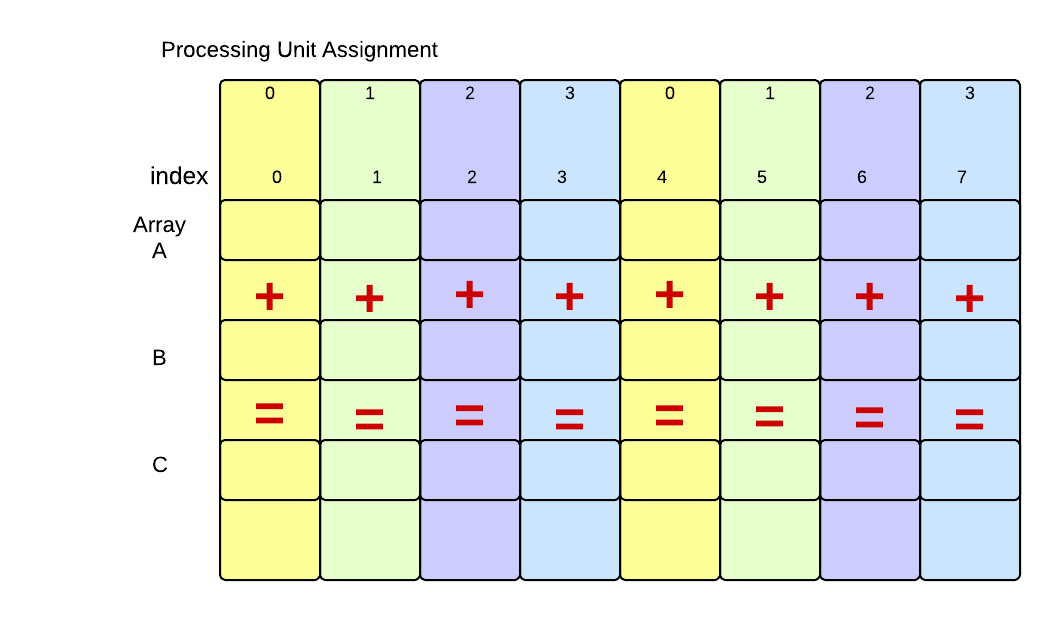
\includegraphics{ChunksOfOne.png}
\end{figure}

This type of decomposition might work fairly well for shared-memory multicore computers using OpenMP, but it doesn't make as much sense for distributed systems using MPI, where the data must be sent from the master process to the other processes in the cluster-- it is much easier to send a consecutive chuank at one time that small lieces over and over again.

Another alternative is to choose a chunk size smaller than n/p and each processing unit will work on then next available chunk.  You can explore these alternatives in OpenMP by looking at documentation for the \textbf{schedule} clause of the pragmaa `omp parallel for'. The CUDA code example called \textbf{VectorAdd/CUDA/VA-GPU-larger.cu} explores this concept.


\section{Questions for reflection}
\label{Decomposition/Variations:questions-for-reflection}
In what situations would MPI on a cluster of computers be advantageous for problems requiring data decomposition?

In what situations would CUDA on a GPU be advantageous for problems requiring data decomposition?

In what situations would OpenMP on a multicore computer be advantageous for problems requiring data decomposition?

In multicore machines, the operating system ultimately schedules threads to run.  Look up what default scheduling of threads to chunks is used in OpenMP if we leave out the \textbf{schedule} clause of the pragmaa `omp parallel for'. Can you find any information or think of why this decomposition is the default?



\renewcommand{\indexname}{Index}
\printindex
\end{document}
